\documentclass[a4paper,12pt]{article} % тип документа

% Поля страниц
\usepackage[left=2.5cm,right=2.5cm, top=2cm,bottom=2cm,bindingoffset=0cm]{geometry}
    
%Пакет дял таблиц   
\usepackage{multirow} 
    
%Отступ после заголовка    
\usepackage{indentfirst}


% Рисунки
\usepackage{subcaption,floatrow,graphicx,calc}
\usepackage{wrapfig}

% Создаёем новый разделитель
\DeclareFloatSeparators{mysep}{\hspace{1cm}}

% Ссылки?
\usepackage{hyperref}
\usepackage[rgb]{xcolor}
\hypersetup{				% Гиперссылки
    colorlinks=true,       	% false: ссылки в рамках
	urlcolor=blue          % на URL
}


%  Русский язык
\usepackage[T2A]{fontenc}			% кодировка
\usepackage[utf8]{inputenc}			% кодировка исходного текста
\usepackage[english,russian]{babel}	% локализация и переносы


% Математика
\usepackage{amsmath,amsfonts,amssymb,amsthm,mathtools, mathrsfs, wasysym}


\begin{document}
\begin{center}
	\footnotesize{ФЕДЕРАЛЬНОЕ ГОСУДАРСТВЕННОЕ АВТОНОМНОЕ ОБРАЗОВАТЕЛЬНОЕ 			УЧРЕЖДЕНИЕ ВЫСШЕГО ОБРАЗОВАНИЯ}\\
	\footnotesize{МОСКОВСКИЙ ФИЗИКО-ТЕХНИЧЕСКИЙ ИНСТИТУТ\\(НАЦИОНАЛЬНЫЙ 			ИССЛЕДОВАТЕЛЬСКИЙ УНИВЕРСИТЕТ)}\\
	\footnotesize{ФАКУЛЬТЕТ ОБЩЕЙ И ПРИКЛАДНОЙ ФИЗИКИ\\}
	\hfill \break
	\hfill\break
	\hfill\break
	\hfill \break
	\hfill \break
	\hfill \break
	\hfill \break
	\hfill \break
	\hfill \break
	\hfill \break
	\hfill \break
	\hfill \break
	\hfill \break
	\hfill \break
	\large{Лабораторная работа № 5.1.3 \\\textbf{Эффект Рамзауэра}}\\
	\hfill \break
	\hfill \break
	\hfill \break
	\begin{flushright}
		Серебренников Даниил\\
		Группа Б02-826м
	\end{flushright}
	\hfill \break
	\hfill \break
	\hfill \break
	\hfill \break
	\hfill \break
	\hfill \break
	\hfill \break
	\hfill \break
	\hfill \break
	\hfill \break
	\hfill \break
\end{center}
\begin{center}
	Долгопрудный, 2020 г.
\end{center}
\thispagestyle{empty}
\newpage
	\textbf{Цель работы:} получить ВАХ эффекта на экране ЭО; измерить расстояние между характерными точками в вольтах; снять ВАХ в статическом режиме; по результатам измерений рассчитать размер электронной оболочки атома, оценить глубину потенциальной ямы и потенциал ионизации атома, заполняющего лампу.

\section{Теоретическая часть}
	К. Рамзауэр исследовал зависимость поперечных сечений упрогого рассеяния электронов (с энергией до 10 ЭВ) на атомах аргона. В результате этих исследований было обнаружено явление, получившее название \textit{эффекта Рамзауэра}.
	
	С точки зрения квантовой теории атом по отношению к электронной волне ведет себя как преломляющая среда с относительным показателем преломления
	\begin{equation*}
		n = \frac{\lambda}{\lambda^\prime} = \sqrt{1-\frac{U}{E}},
	\end{equation*}
	где $U$, $E$ -- соответственно потенциальная и полная энергии электрона внутри атома.
	
	Будем считать, что электрон рассеивается на одномерной прямоугольной потенциальной яме конечной глубины. Такая модель является хорошим приближением для атомов тяжелых инертных газов, отличающихся наиболее компактной структурой и резкой внешней границей. Решение задачи о прохождении частицы с энергией $E$ над потенциальной ямой шириной $l$ и глубиной $U_0$ не составит труда найти из уравнения Шредингера:\\
	\begin{equation*}
		\psi^{\prime\prime}+k^2\psi=0, \ \text{где}\
		k^2 =\begin{cases}
			2mE/\hbar^2 & x<0, x>l\\
			(2mE+U_0)/\hbar^2 & 0<x<l
		\end{cases}.
	\end{equation*}
	Коэффициент прохождения равен отношению квадратов амплитуд прошедшей и падающей волн и определяется выражением:
	\begin{equation*}
		\frac{1}{D} = 1 + \frac{U_0^2}{4E(E+U_0)}\sin^2(k_2l).
	\end{equation*}
	Минимум последнего выражения отвечает квантовому аналогу просветления оптики, так как при выполнении условия
	\begin{equation*}
		\tag{$\star$}
		\label{eq:uslovie}
		\sqrt{\frac{2m(E+U_0)}{\hbar^2}}l = \pi n, \ n\in\mathbb{N},
	\end{equation*}
	коэффициент прохождения частицы над ямой становится равным единице, то есть достигает своего максимального значения.
	Отметим, что условие~(\ref{eq:uslovie}) легко получить, рассматривая интерференцию электронов волн де Бройля в атоме:\\
	\begin{itemize}
		\item
			Условие первого интерференционного максимума:
			\begin{equation}
				\label{eq:1}
				2l = \frac{h}{\sqrt{2m(E_1+U_0)}}.
			\end{equation}
		\item
			Условие первого интерференционного минимума:
			\begin{equation}
				\label{eq:2}
				2l =\frac{3}{2} \frac{h}{\sqrt{2m(E_1+U_0)}}.
			\end{equation}			
	\end{itemize}

	Решая совместно уравнения~(\ref{eq:1}, \ref{eq:2}) можно получить:
	\begin{equation}
		\label{eq:l}
		l = \frac{h\sqrt{5}}{\sqrt{32m(E_2-E_1)}}.
	\end{equation}
	Понятно, что энергии $E_1$ и $E_2$ соответствуют энергиям электронов, прошедших разность потенциалов $V_1$ и $V_2$, то есть $E_1 = eV_1$ и $E_2 = eV_2$. 
	
	По измеренным величинам $E_1$ и $E_2$, используя формулы~(\ref{eq:1}, \ref{eq:2}), можно рассчитать эффективную глубину потенциальной ямы атома:
	\begin{equation}
		\label{eq:U_0}
		U_0 = \frac{4}{5}E_2 - \frac{9}{5}E_1
	\end{equation}

	Согласно квантовой механике зависимость вероятности рассеяния электрона от его энергии можно определить из соотношения:
	\begin{equation}
		\label{eq:w}
		w(U) = -\frac{1}{C}\ln \frac{I(U)}{I_0},
	\end{equation}
	где $I_0$ -- ток катода, а $C$ -- некторая постоянная.
	
	



\section{Экспериментальная установка}
	В нашей работе для изучения эффекта Рамзауэра используется тиратрон ТГ3-01/1.3Б, заполненный инертным газом. Схематическое изображение тиратрона и его конструкция приведены на рис.~\ref{pic1}.
	
	Принципиальная схема установки для изучения эффекта Рамзауэра приведена на рис.~\ref{pic2}. На лампу Л подаётся синусоидальное напряжение частоты 50 Гц от источника питания ИП, С -- стабилизированный блок накала катода; исследуемый сигнал подаётся на электронный осциллограф (ЭО); цифрами обозначены номера ножек лампы.
	
	\thisfloatsetup{floatrowsep=mysep}	
	\begin{figure}[h!]
		\ffigbox{
			\begin{subfloatrow}[2]
				\ffigbox[\FBwidth]{\caption{}}%
				{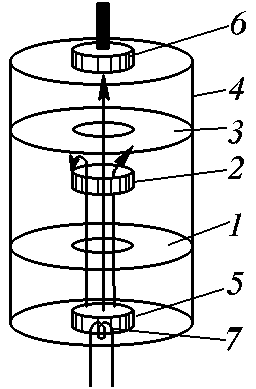
\includegraphics[width=3cm,height=4.5cm]{pic1}{\label{pic1}}}
				\ffigbox[\FBwidth]{\caption{}}%
				{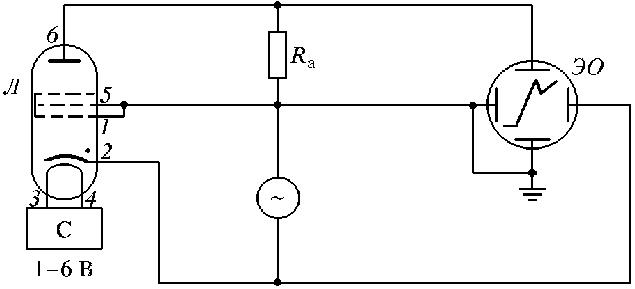
\includegraphics[width=7cm,height=4cm]{pic2}{\label{pic2}}}         
			\end{subfloatrow}
		}
		{\caption{Экспериментальная установка.}}
	\end{figure}
	
	Схема экспериментальной установки, изображённая на рис.~\ref{pic2} в нашей работе конструктивно осуществлена следующим образом. Лампа-тиратрон ТГ3-01/1.3Б, заполненная инертным газом, расположена непосредственно на корпусе блока источника питания (БИП). Напряжение к электродам лампы подаётся от источников питания, находящихся в корпусе прибора. Регулировка напряжения и выбор режима работы установки производится при помощи ручек управления, выведенных на лицевую панель БИП.
	
	
	\newpage
	\section{Экспериментальные данные}
		
	
	
		\floatsetup[table]{capposition=top}	
		\begin{table}[H]
			\caption{Некоторые измеряемые величины и их погрешность.}
			\label{table:parametr}
			\begin{tabular}{|c|c|c|c|c|c|c|}
				\hline
				& $V$, В & $E_1$, эВ & $E_2$, эВ & $E_\text{ион.}$, эВ & $U$, В & $I$, мА \\ \hline
				Величина          & 2,65   & 1,9       & 7,0       & 12,5                & 5,0    & 1,00    \\ \hline
				Погрешность       & 0,02   & 0,1       & 0,5       & 0,5                 & 0,1    & 0,05    \\ \hline
				$\varepsilon$, \% & 1,0    & 5,3       & 7,1       & 4,0                 & 2,0    & 5,0     \\ \hline
			\end{tabular}
		\end{table}
		
		\floatsetup[table]{capposition=top}	
		\begin{table}[H]
			\caption{Результаты измерений в динамическом режиме.}
			\label{table:exp1}
			\begin{tabular}{|c|c|c|c|}
				\hline
				$V$, В & $E_1$, эВ & $E_2$, эВ & $E_\text{пробоя}$, эВ \\ \hline
				2,65   & 1,9       & 7,0       & 12,5                \\ \hline
				2,34   & 1,4       & 7,0       & -                   \\ \hline
			\end{tabular}
		\end{table}
		
		
	
		\floatsetup[table]{capposition=top}	
		\begin{table}[H]
			\caption{Результаты измерений в статическом режиме.}
			\label{table:exp2}
			\begin{tabular}{|c|c|c|c|c|c|}
				\hline
				\multicolumn{2}{|c|}{2,17 В} & \multicolumn{2}{c|}{2,42 В} & \multicolumn{2}{c|}{2,62 В} \\ \hline
				$U$, В        & $I$, мА       & $U$, В       & $I$, мА       & $U$, В       & $I$, мА       \\ \hline
				1,0           & 0,04          & 1,0          & 0,10          & 1,0          & 0,19          \\ \hline
				2,0           & 0,23          & 2,0          & 0,79          & 2,0          & 1,68          \\ \hline
				3,0           & 0,08          & 2,0          & 0,89          & 1,8          & 1,80          \\ \hline
				4,0           & 0,05          & 1,9          & 0,98          & 1,4          & 1,42          \\ \hline
				7,1           & 0,03          & 1,6          & 1,16          & 1,7          & 1,82          \\ \hline
				8,0           & 0,03          & 3,0          & 0,31          & 2,0          & 1,73          \\ \hline
				8,3           & 0,03          & 4,0          & 0,19          & 2,2          & 1,59          \\ \hline
				9,0           & 0,03          & 5,0          & 0,14          & 0,1          & 0,00          \\ \hline
				11,7          & 0,06          & 6,0          & 0,12          & 3,1          & 0,85          \\ \hline
				1,6           & 0,36          & 7,1          & 0,12          & 4,0          & 0,53          \\ \hline
				1,7           & 0,34          & 6,8          & 0,12          & 5,0          & 0,40          \\ \hline
				1,4           & 0,33          & 8,0          & 0,13          & 6,8          & 0,34          \\ \hline
				&               & 9,0          & 0,15          & 6,6          & 0,35          \\ \hline
				&               & 11,7         & 0,29          & 6,3          & 0,35          \\ \hline
				&               &              &               & 5,8          & 0,37          \\ \hline
				&               &              &               & 7,2          & 0,35          \\ \hline
				&               &              &               & 7,4          & 0,35          \\ \hline
				&               &              &               & 7,7          & 0,36          \\ \hline
				&               &              &               & 8,2          & 0,38          \\ \hline
				&               &              &               & 9,4          & 0,45          \\ \hline
				&               &              &               & 11,5         & 0,79          \\ \hline
			\end{tabular}
		\end{table}
	
	\newpage
	\section{Обработка результатов}
		По результатам измерений в динамическом режиме (табл. \ref{table:exp1}) рассчитаем размер электронной оболочки атома инертного газа, заполняющего лампу, используя формулы (\ref{eq:1}~-~\ref{eq:l}). Погрешности оценим по формулам:
		\begin{equation*}
			\sigma_{l_1} = l_1 \frac{\sigma_{E_1}}{E_1}, \ \sigma_{l_2} = l_2 \frac{\sigma_{E_2}}{E_2}, \ \sigma_{l_3} = l_3 \frac{\sigma_{E_1}+\sigma_{E_2}}{E_2-E_1}.
		\end{equation*}
		Эффективную глубину потенцаиальной ямы $U_0$ можно оценить по формуле~(\ref{eq:U_0}), причем
		\begin{equation*}
			\sigma_{U_0} = \frac{4}{5}\sigma_{E_2}+\frac{9}{5}\sigma_{E_1}.
		\end{equation*}
		Результаты вычислений представлены в таблицах:
		\begin{table}[h!]
			\begin{floatrow}
				\ttabbox[\FBwidth]{\caption{$l_1,l_2,l_3, U_0$.}\label{l1-3,U0}}%
				{\begin{tabular}{|c|c|c|c|c|}
						\hline
						$V$, В & $l_1$, пм & $l_2$, пм & $l_3$, пм & $U_0$, эВ \\ \hline
						2,65   & 290       & 300       & 300       & 2,2       \\ \hline
						2,34   & 310       & 300       & 290       & 3,1       \\ \hline
				\end{tabular}}
				\ttabbox[\FBwidth]{\caption{$l, U_0$.}\label{lambda}}%
				{\begin{tabular}{|c|c|c|}
						\hline
						& $l$, пм        & $U_0$, эВ     \\ \hline
						Эксперимент & $300 \pm 30$ & $2,6 \pm 0,6$ \\ \hline
						Справочник  & 280          & 2,5           \\ \hline
				\end{tabular}}        
			\end{floatrow}
		\end{table}
	
		Отметим, что в качестве табличного значения размера электронной оболочки был взят удвоенный ковалентный радиус ксенона, так как на эксперименте пробой тиратрона наблюдался при $E_\text{пробоя} = (12,5 \pm 0,5)$ эВ, что примерно есть ионизационный потенциал ксенона 12,1 эВ.
		
		По результатам измерений в статическом режиме~(табл. \ref{table:exp2}) построим методом интерполяции сплайнами Акима графики завивисимости $I = I(U)$ при различных напряжениях накала $V$ и зависимости вероятности рассеяния $w$ электрона атомом ксенона от его энергии (напряжения на катоде $U$) с точностью до константы $C$.
		\begin{figure}[h!]
			\begin{floatrow}
				\ffigbox[\FBwidth]{\caption{ВАХ тиратрона в стат. режиме.}\label{fig:static_mode}}%
				{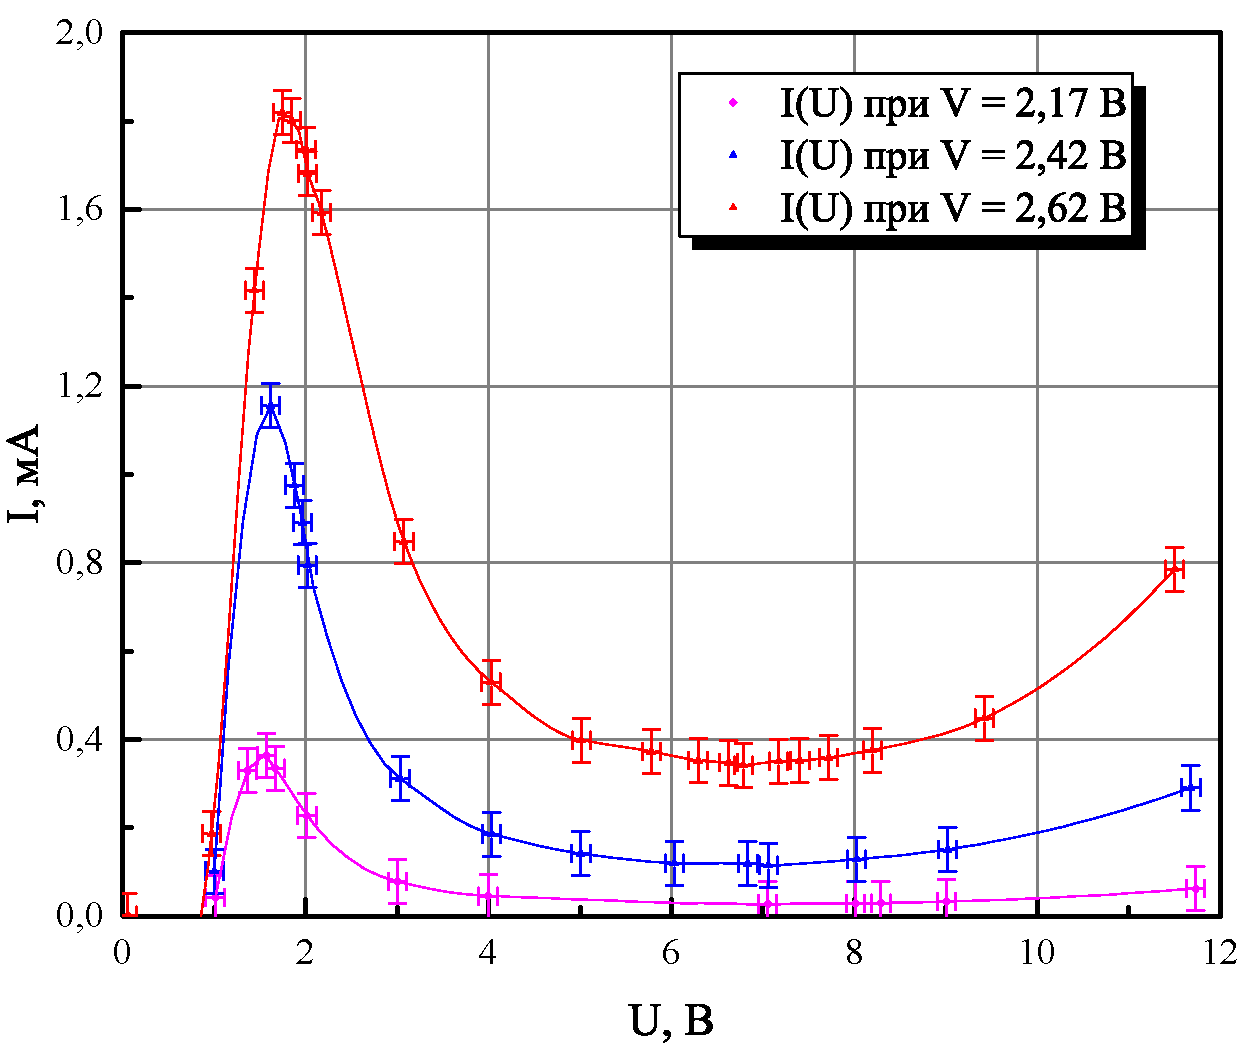
\includegraphics[width=8cm,height=7cm]{graph1.pdf}}
				\ffigbox[\FBwidth]{\caption{Вероятность рассеяния электрона.}\label{fig:W}}%
				{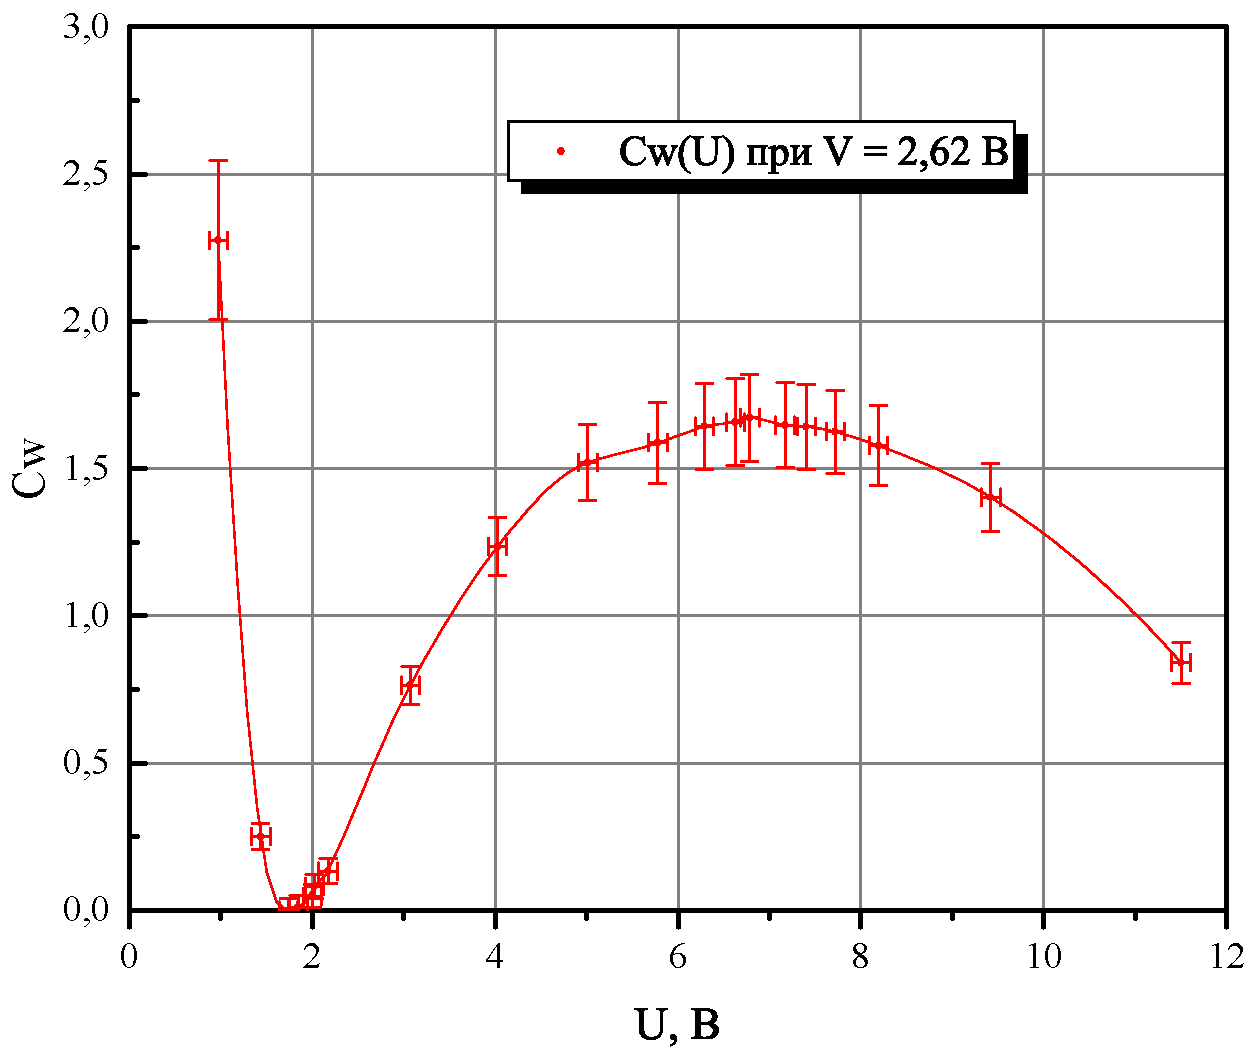
\includegraphics[width=8cm,height=7cm]{graph2.pdf}}     
			\end{floatrow}
		\end{figure}
	
		Ясно, что при $V = 2,65$ В ток катода $I_0 =(1,82 \pm 0,05)$ мА есть максимум на ВАХ тиратрона, а 
		\begin{equation*}
			\sigma_{Cw} = \sigma_I \sqrt{\frac{1}{I^2} + \frac{1}{I_0^2}}.
		\end{equation*}
		

\newpage
\section{Обсуждение результатов и выводы}
	В ходе лабораторной работы мы наблюдали ВАХ тиратрона в динамическом режиме (рис.~\ref{photo1}) при различных напряжениях накала, причем по напряжению пробоя определили, что используемый в эксперименте инертный газ состоит из атомов ксенона. Действительно, энергия ионизации ксенона -- 12,1 эв, а $E_\text{пробоя} = (12,5 \pm 0,5)$ эВ. Более того, нам удалось вычислить размер электронной оболочки атома ксенона $l = 300$ пм с точностью в 10\%, который в пределах погрешности совпадает с табличным значением его удвоенного ковалентного радиуса -- 280 пм. Также была вычислена эффективная глубина потенциальной ямы ксенона $U_0 = 2,6$ эВ с ошибкой в 24\%.
	
	Вольт-амперная характеристика тиратрона в статическом режиме (рис.\ref{fig:static_mode}) имеет вид, который находится в согласии с квантовой теорией. Электрон, обладая волновыми свойствами, способен <<интерферировать сам с собой>> при рассеянии на атоме, тем самым усиливая или ослабевая анодный ток. Энергии электрона (напряжения на катоде) при которых наблюдаются максимумы или минимумы в статическом режиме примерно совпадают со значениями, полученными при измерениях в динамическом режиме. Заметим, что максимумы несколько смещаются вправо по рис.~\ref{fig:static_mode} при увеличении напряжения накала, что может быть обусловлено наличием контактной разности потенциалов.
	
	Проанализируем вид зависимости $w = w(U)$, представленной на рис.~\ref{fig:W}, при напряжении накала $V = 2,62$ В с точностью до константы $C$. На графике в диапазоне от 1В до 12В отчетливо видны максимум и минимум, что подтверждает справдливость эффекта Рамзауэра -- эффективное сечение реакции сильно зависит от энергии электрона. Однако видно, что при достаточно малых энергиях электрона погрешность вероятности сильно возрастает, что неудивительно, ведь из формулы (\ref{eq:w}) видно, что $w\rightarrow +\infty$ при $U\rightarrow0$ (этот предел не зависит от нормировачной константы $C$), что противоречит физической реальности. Можно сделать вывод, что формула (\ref{eq:w}) имеет границы применимости: энергия электрона $E \geq 1$ эВ. При меньших энергиях электрон может испытывать другие квантовые эффекты: рассеяние медленных частиц, резонансное рассеяние при малых энергиях.

\newpage
\section*{Приложение}
	\thisfloatsetup{floatrowsep=mysep}	
	\begin{figure}[h!]
		\ffigbox{
			\begin{subfloatrow}[2]
				\ffigbox[\FBwidth]{\caption{}}%
				{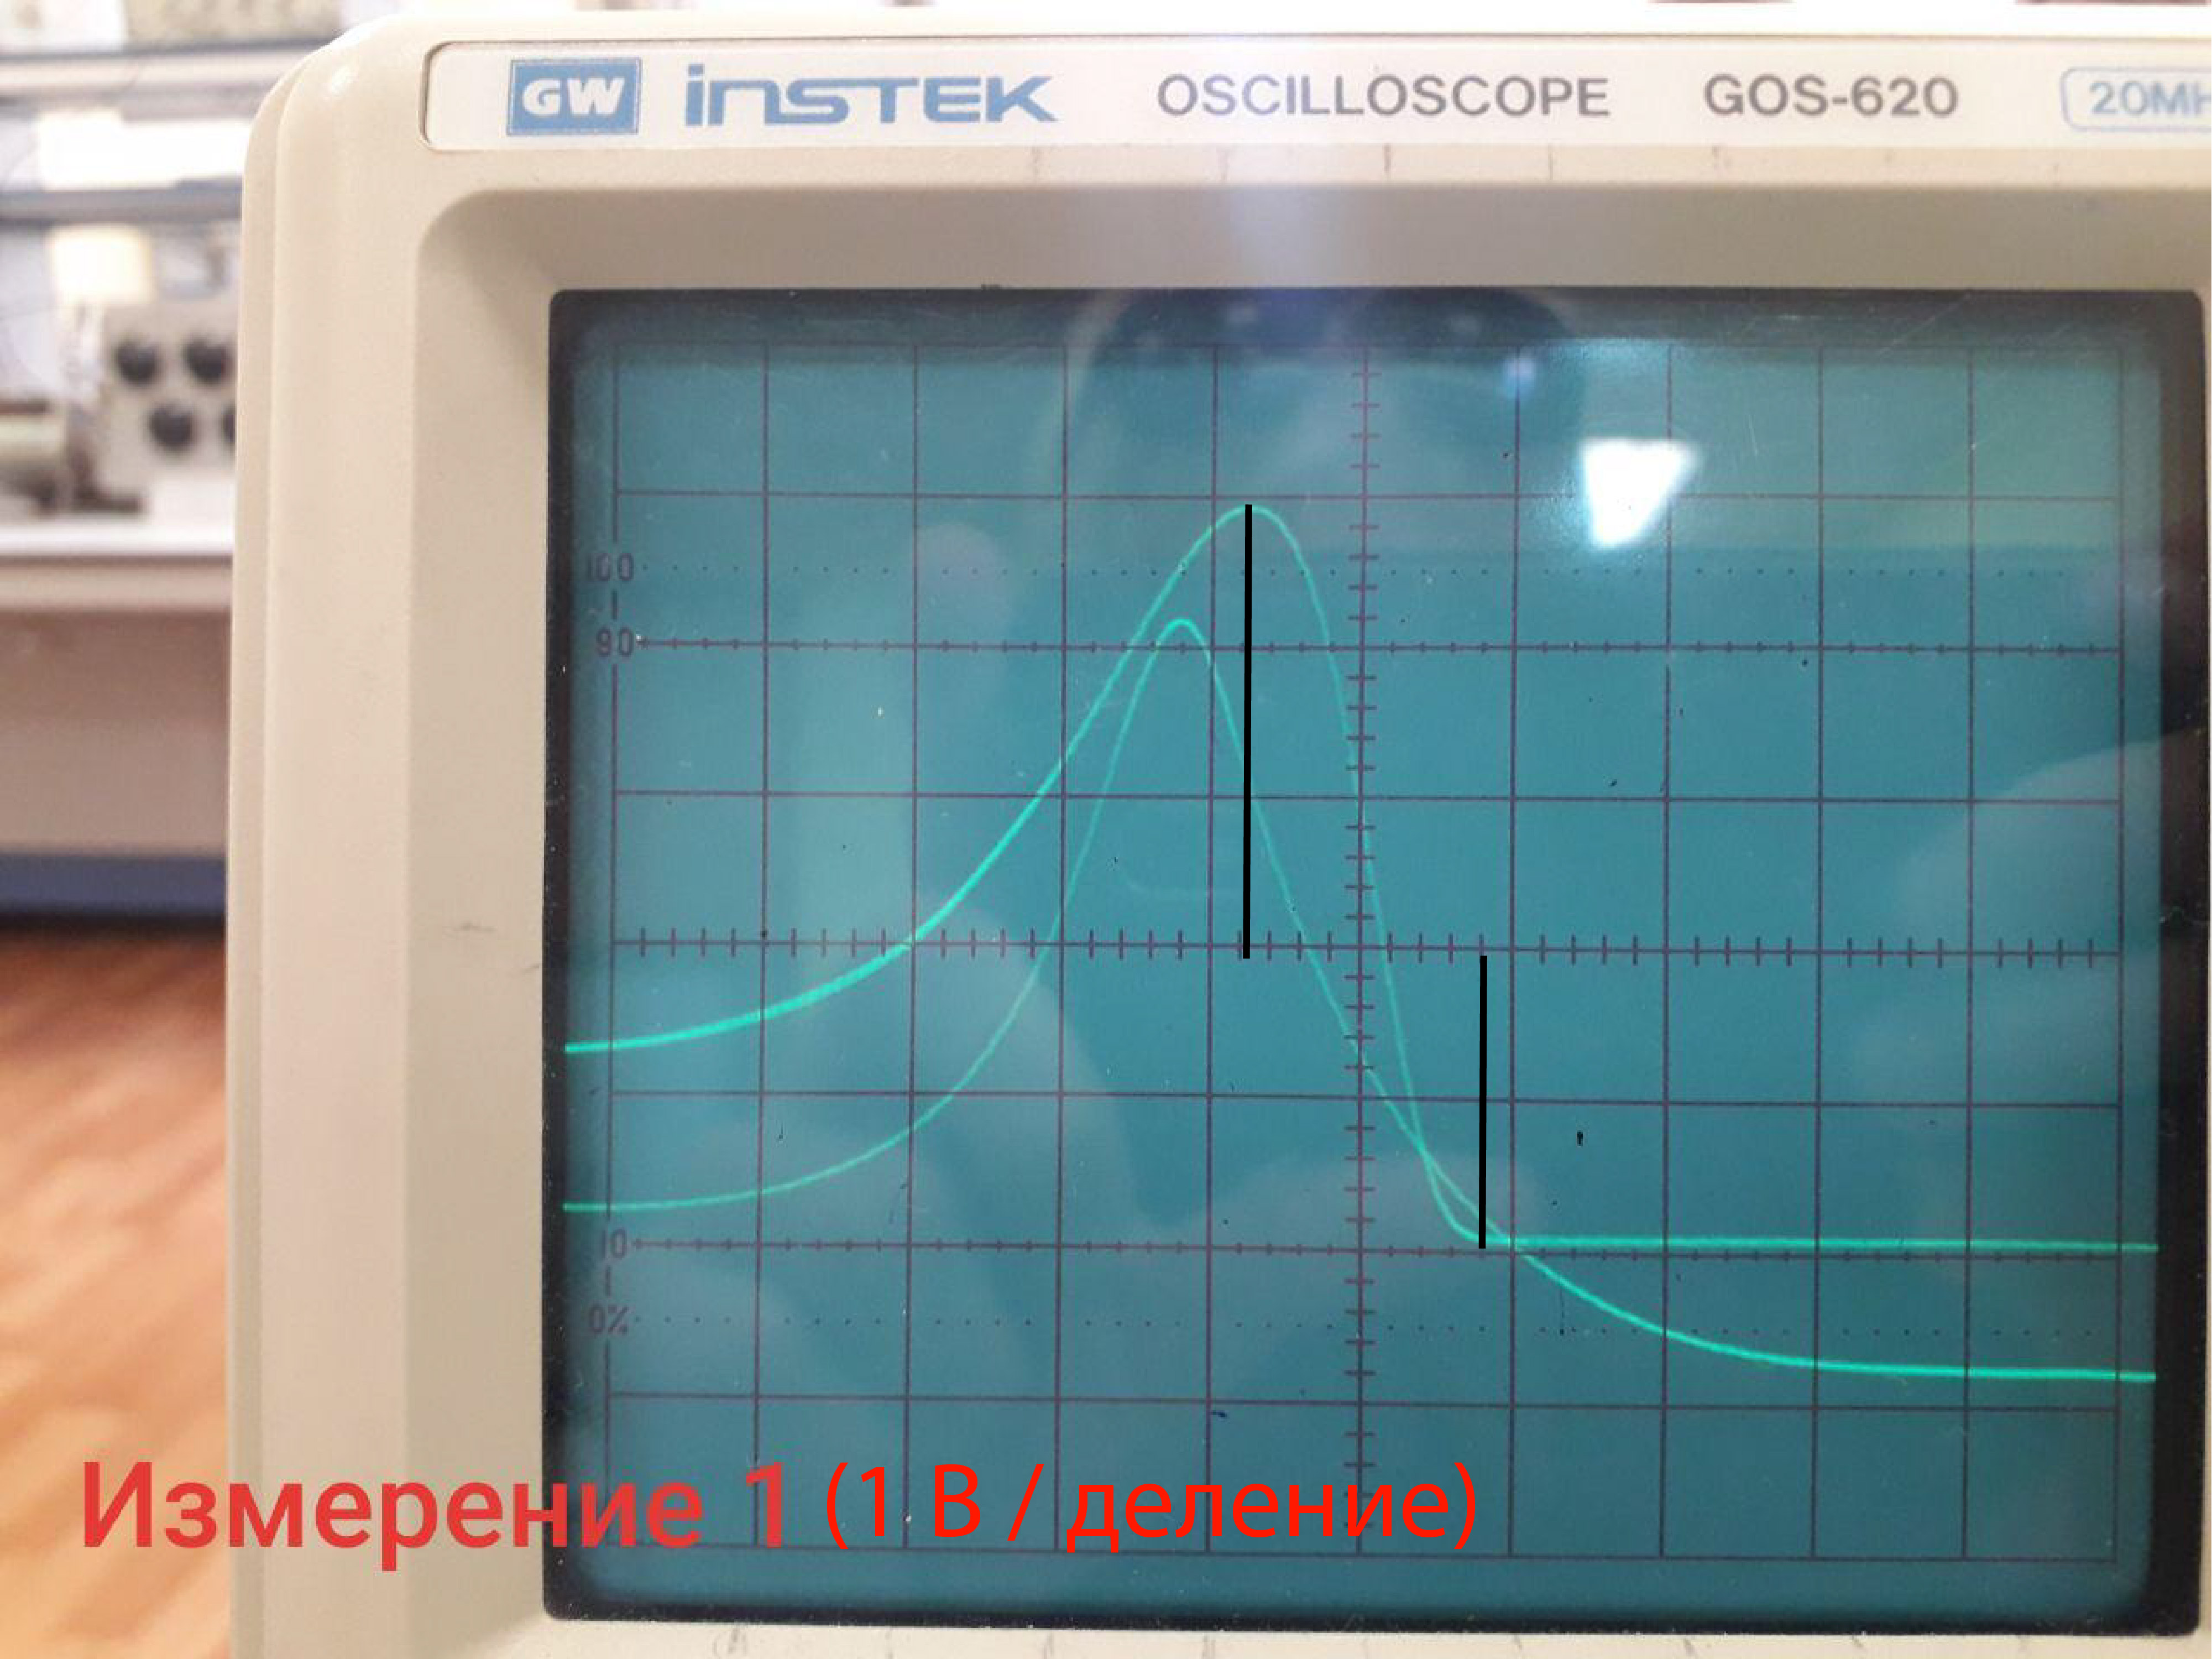
\includegraphics[scale=0.25]{photo1.jpg}{\label{photo1}}}
				\ffigbox[\FBwidth]{\caption{}}%
				{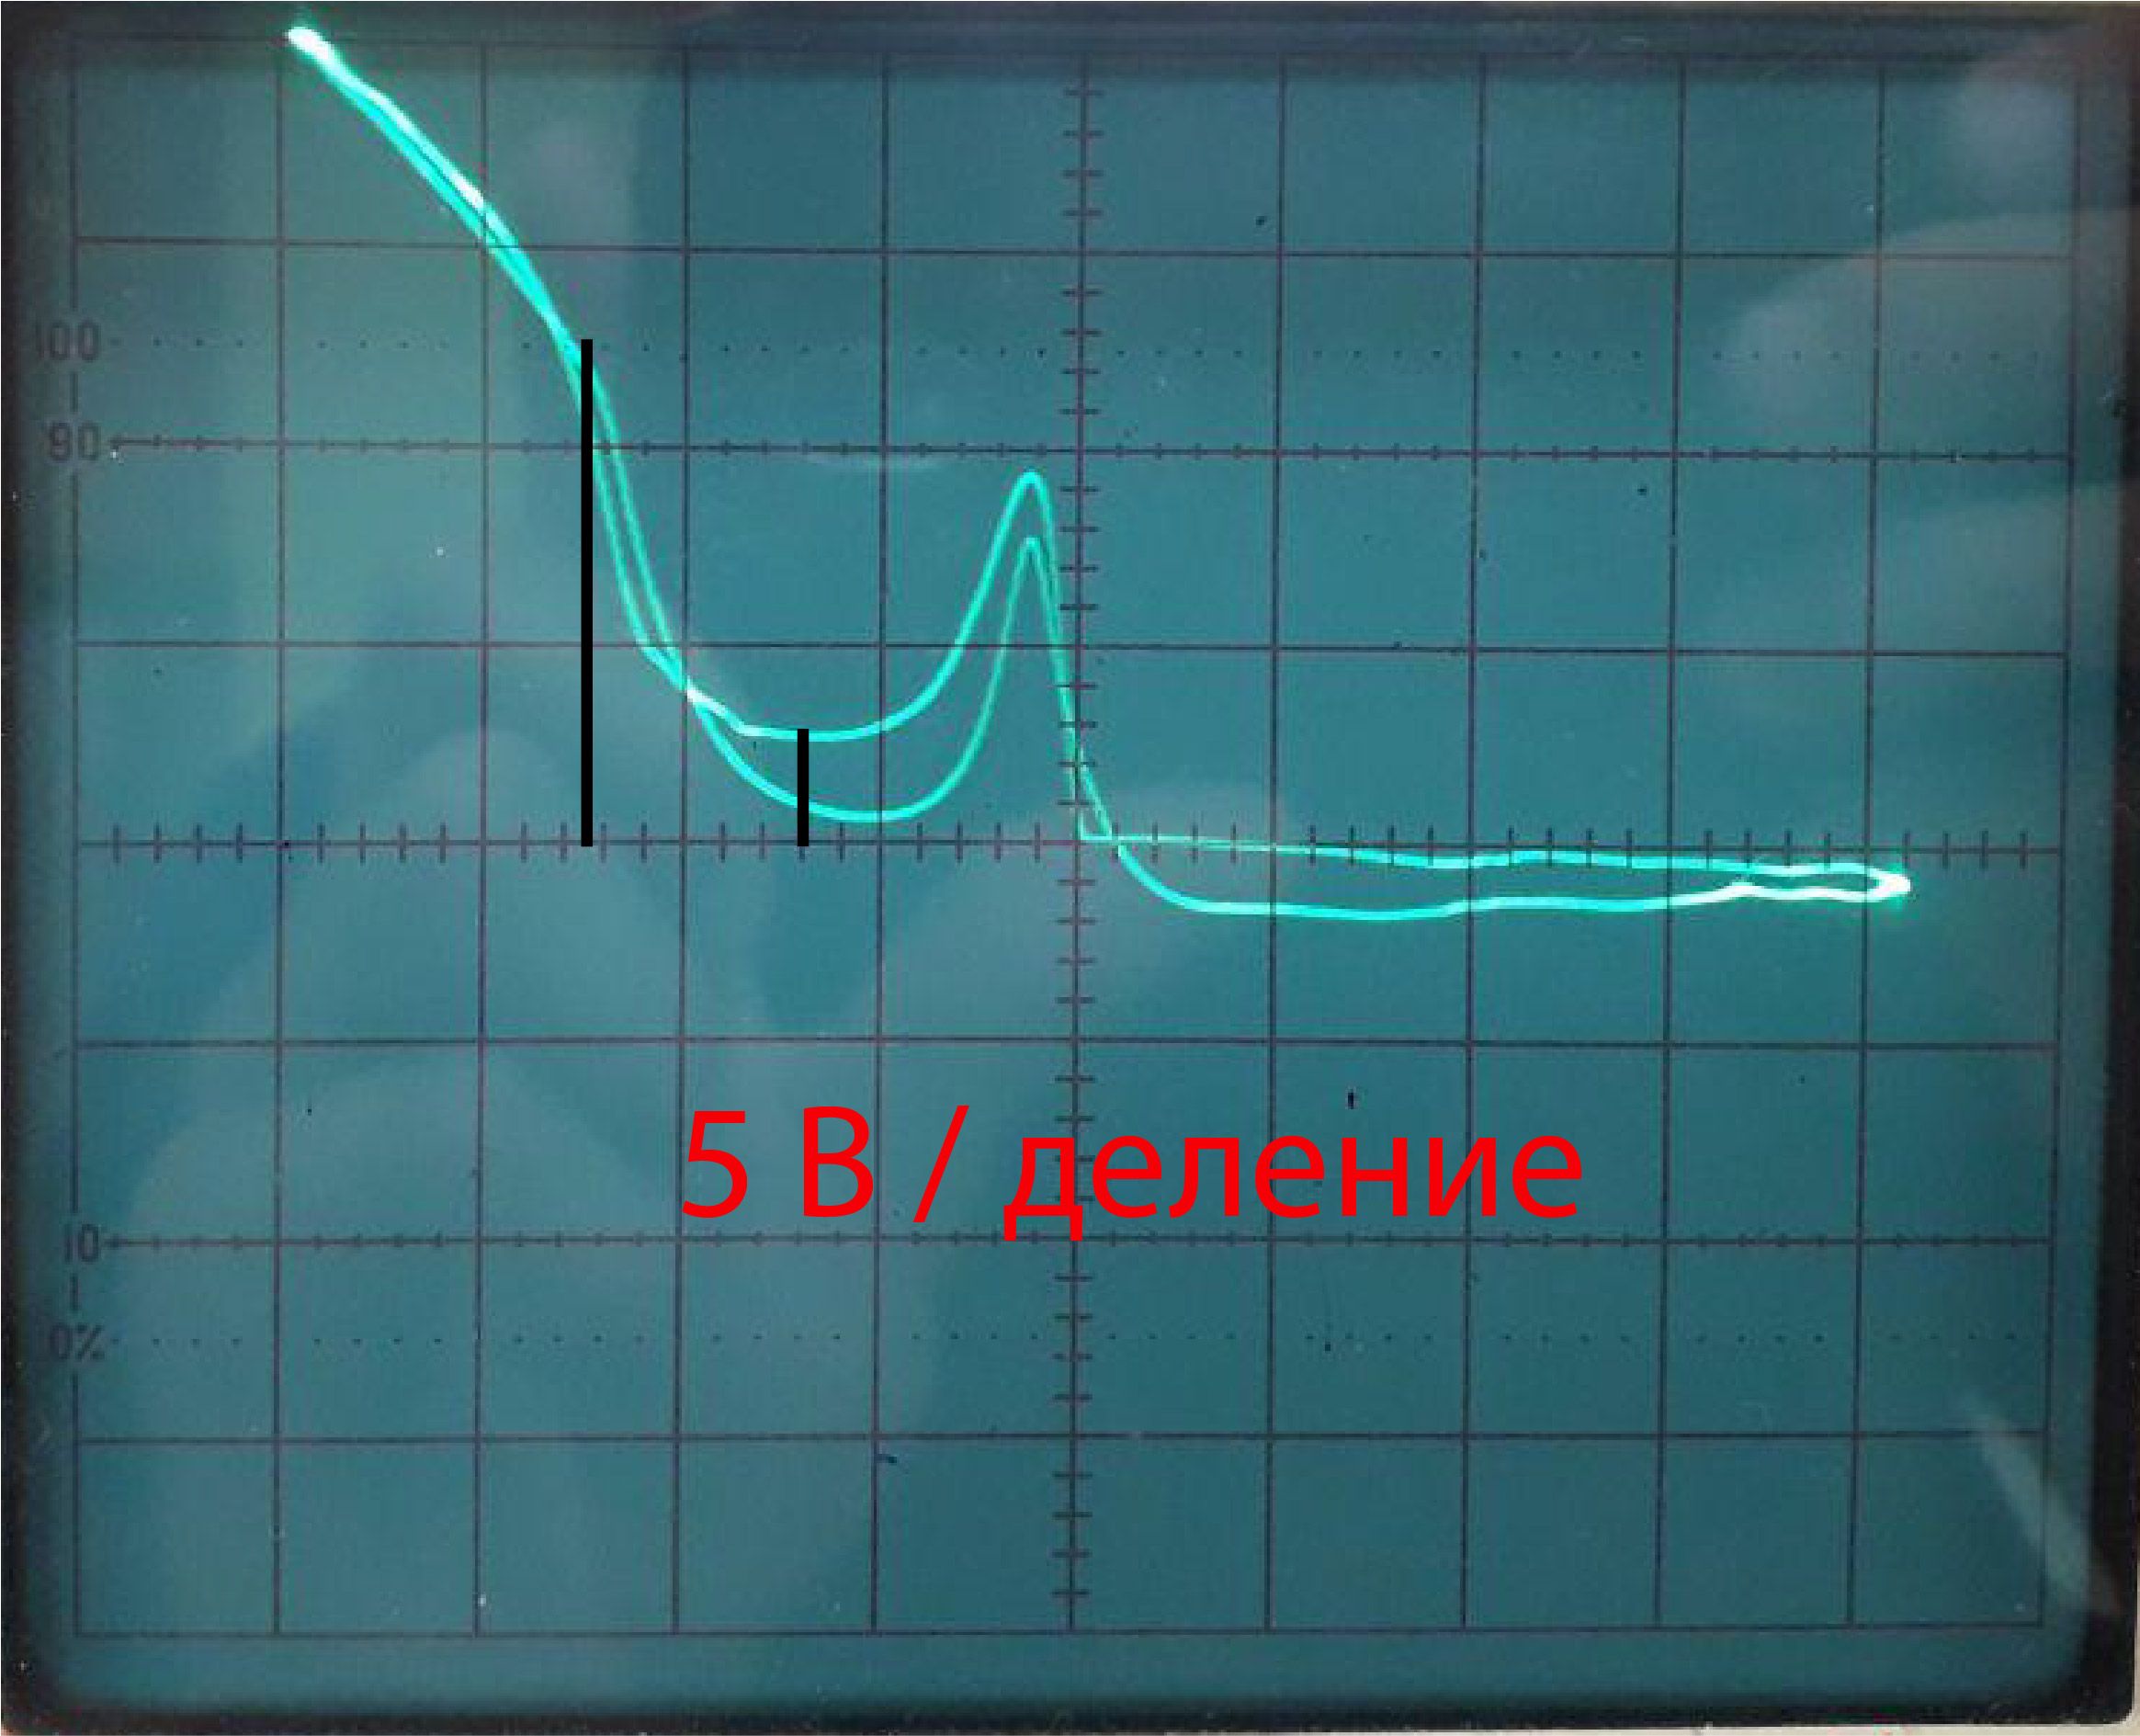
\includegraphics[scale=0.4]{photo2.jpg}{\label{photo2}}}         
			\end{subfloatrow}
		}
		{\caption{ВАХ тиратрона в динамическом режиме при $V = 2,65$ В.}}
	\end{figure}

\end{document}